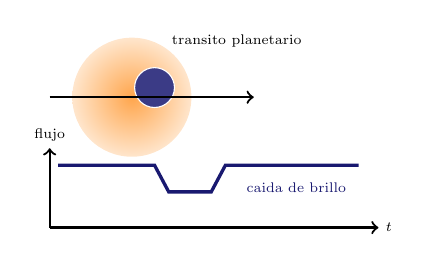
\begin{tikzpicture}[scale=0.72,transform shape]
\shade[inner color=orange!70,outer color=orange!20] (-1.55,0.75) circle (1.05);
\node[circle,fill=MidnightBlue!85,draw=white,minimum size=20pt] at (-1.15,0.92) {};
\draw[thick,->] (-3.0,0.75) -- (0.6,0.75);
\draw[->,thick] (-3.0,-1.55) -- (2.8,-1.55) node[right,font=\scriptsize] {$t$};
\draw[->,thick] (-3.0,-1.55) -- (-3.0,-0.15) node[above,font=\scriptsize] {flujo};
\draw[very thick,MidnightBlue] (-2.85,-0.45) -- (-1.15,-0.45) -- (-0.9,-0.92) -- (-0.15,-0.92) -- (0.1,-0.45) -- (2.45,-0.45);
\node[font=\scriptsize] at (0.3,1.75) {transito planetario};
\node[font=\scriptsize,MidnightBlue] at (1.35,-0.85) {caida de brillo};
\end{tikzpicture}
